\documentclass{beamer}
\usepackage[T1]{fontenc}
\usepackage[polish]{babel}

\usetheme{Madrid} % Wybierz motyw prezentacji

\title{Charakterystyka i różnice między modelem koncepcyjnym, logicznym i fizycznym bazy danych}
\author{Bernard Pokorski}
\date{30.11.2023}

\begin{document}

\begin{frame}
\titlepage % Strona tytułowa
\end{frame}

\begin{frame}
\frametitle{Ćwiczenie wstępne}
Cel ćwiczenia:
\begin{enumerate}
    \item \textbf{Zrozumienie różnic pomiędzy modelmi:} \\ koncepcyjnym, logicznym i fizycznym baz danych
\end{enumerate}
\end{frame}

\begin{frame}
    \frametitle{Przykład}
    Załóżmy, że jesteśmy pracownikiem biblioteki i chcemy usprawnić działanie naszej biblioteki.
    W tym celu chcemy skatalogować wszystkie książki w naszej bibliotece.
    Chcemy: 
    \begin{enumerate}
    \item przechowywać bardziej szczegółowe informacje na temat autorów np.: \\ \textbf{\textit{daty ich urodzenia, kraj z którego pochodzą}}
    \item przechowywać informacje o książkach np.:\\ \textbf{\textit{tytuł, kto jest ich autorem, kto jest wydawcą}}
    \item przechowywać dane kontaktowe do konkretnego wydawnictwa np.:\\ \textbf{\textit{numer telefonu, adres}}
\end{enumerate}
\end{frame}

\begin{frame}
    \frametitle{Opisanie związków}
    Na potrzeby biblioteki przyjmujemy, że mówiąc książka mamy na myśli fizyczny egzemplarz
    \begin{block}{Książka - autor}
        Książka jest napisana przez jednego lub więcej autorów, a autor może napisać jedną lub więcej książek.
    \end{block}
    \begin{block}{Książka - wydawnictwo}
        Pojedyncza książka może być wydana tylko przez jedno wydawnictwo 
    \end{block}
\end{frame}

\begin{frame}
    \frametitle{Model koncepcyjny}
   To co przed chwilą zrobiliśmy nazywa się \textbf{Analizą biznesową}. \\
   Przy wykorzystaniu \textbf{Diagramu Związków Encji (ERD)} spróbujemy przedstawić naszą koncepcję 
\end{frame}

\begin{frame}
    \frametitle{Model koncepcyjny}
    \begin{figure}
        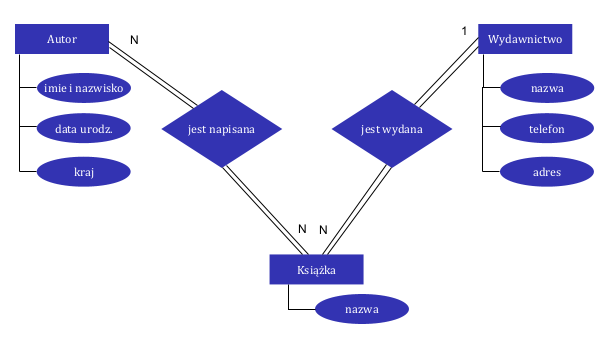
\includegraphics[width=1\textwidth]{erd.png}
        \caption{Przykładowy diagram związków encji}
    \end{figure}
\end{frame}

\begin{frame}
    \frametitle{Model logiczny}
    Skoro mamy już konecpcyjny model bazy danych czas pomyśleć\\ 
    \textit{jak moglibyśmy przełożyć na konkretny silnik bazodanowy}\\
    \textbf{W zależności od typu bazy danych model logiczny może być różny!} 
    Na przykład dla baz relacyjnych np. MySQL tworzone są klucze podstawowe i obce, a związki wiele do wielu są przedstawiane jako tabele.
    \begin{block}{Przykładowe silniki bazodanowe}
        \begin{enumerate}
        \item Silniki relacyjnych baz danych (RDBMS): \textit{MySQL, PostgreSQL}
        \item Silniki NoSQL: \textit{MongoDB, Cassandra, Redis}
        \item Inne silniki specjalizowane: \textit{Elasticsearch, Neo4j}  
        \end{enumerate}
    \end{block}
\end{frame}

\begin{frame}
    \frametitle{Model fizyczny}
    Pozostaje pytanie jak te dane w efektywny sposób przechowywać?\\
    Na tym etapie postają elementu potrzebne do efektywnego zarządzania bazą danych.\\
    \begin{block}{Przykładowo}
    W relacyjnych bazach danych dodawane są indeksy i określane konkretne parametry pól np. VARCHAR(2137), TEXT, INT
    \end{block}

\end{frame}

\begin{frame}
    \frametitle{Modele bazy danych}
    \begin{block}{Model koncepcyjny}
        Skupia się na ogólnych potrzebach biznesowych i jest abstrakcyjny. \\
        To znaczy, że nie zawiera \textbf{żadnych} informacji związanych z implementacją. \\ 
        \textbf{\textcolor{red}{Przedstawia jedynie encje i związki między nimi}}
    \end{block}
    \begin{block}{Model logiczny}
        Przetwarza model koncepcyjny na poziomie bardziej technicznym, używając schematu danych.
        W zależności od wybranej bazy (a w szczególności typu) danych modele logiczne będą się od siebie rózniły.
    \end{block} 
    \begin{block}{Model fizyczny}
        Definiuje, w jaki sposób dane są przechowywane na poziomie fizycznym, uwzględniając specyfikę bazy danych.
    \end{block}
\end{frame}

\end{document}
